\chapter{Science Is Elementary 2}

% \begin{figure}[H]
%     \centering
%     \includegraphics[width=\textwidth/2]{./Games/EveryChildCanSucceed/Images/EveryChildCanSucceed7CD.png}
%     \caption{Every Child Can Succeed 7 CD}
% \end{figure}

The second of the Science Is Elementary games published and released by The Lightspan Partnership for the PlayStation 1.

Science Is Elementary 2 features three video programs:

\begin{itemize}
    \item Let's Explore Water
    \item Let's Explore Tools and Work
    \item Let's Explore Magnets
\end{itemize}

\clearpage
\newpage

\section{Let's Explore Water}

\subsection{Audio Summary}

In "Let's Explore Water", we discover the properties of water, identify water sources and water's importance to all living things. In the exploration, we investigate how water freezes and melts.

\subsection{Transcription}

Girl 1: You know what? Water's wet.

Girl 2: You see, you can see through water.

Girl 3: You can pour water.

Girl 4: Some things flow in water.

Girl 5: Water mixes with lots of things.

Girl 6: Water can flow downhill.

Boy 1: Look! Water splashes!

Young Girl: You turn on the faucet and wow, water. But water can be found in so many places. Where else can you find water? Mmm, tastes good. We all use water. How do you use water?

(transition to a different scene)

Young Girl: All living things need water. Watch our raindrop and see.

Young Girl (voice over): Everything needs water to sip. My flower's in bloom, it's thirsty I assume. My dog's bowl is dry. I sigh, oh my. My goldfish is sinking, it needs fluid I'm thinking. And this empty glass is no help for thirsty laughs. To all of these, give them water please. On every street and lane, what we really need is rain. Hey cloud, show us your power to provide a shower. Ah, these drops and drips give us wonderful sips. For living things like us, rain is glorious.

(transition to a different scene)

Young Girl (voice over): What do these children and their teacher discover about ice?

Teacher: I'm going to hand each of you a piece of ice and I want you to just hold it in your hands. You're each going to get one and notice what's happening to it. Okay, why do you suppose -

Kristin: It's all slippery too!

Teacher: It's slippery, yes! [inaudible] It's very slippery. Go ahead Daniel, get it! Ice is slippery. Does it get more slippery or less slippery do you think?

Kristin: I think it gets more slippery.

Teacher: More slippery. All right, yeah, very good. Okay, what I'm going to give you now as you hold it, I'm going to give you a jar and you're going to get to hold your ice over the jar. What are we going to collect in this jar, you suppose?

Daniel: The water.

Teacher: The water, excellent, we're going to collect water.

Christian: Augh man, now it's dripping mine.

Teacher: There you go, let it drip.

Daniel: Cold.

Teacher: Yeah? Let's go, let it drip into your cup here. Keep it still.

Daniel: No, mine is getting a whole bunch of water.

Christian: Me too.

Teacher: Now why do you suppose these ice cubes are melting?

Christian: Because it's hot.

Teacher: It's hot or hard?

Christian: Hot.

Teacher: Yeah, your hands are making it warm, and when the ice cube gets warm, what happens to it?

Christian: It melts.

Teacher: And it's getting all this water into our jar. What's happening?

Kristin: You close your hands and the air gets warmer and it melts.

Teacher: Okay. Oh look at these ice cubes now. Put them out in your hand and let's look at all of them. Interesting. Look at how this one is just\dots Do you see anything that's different about any of them? You notice the bubbles in yours. What do you notice?

Kristin: Um, it's, they're smaller.

Teacher: They're small.

Kristin: Mines is real small.

Teacher: Yours is very small, real small. That's true.

Christian: [inaudible]

Teacher: Look at what we've done. It started off like this, and with just a little bit of time, look at what has happened.

Daniel: It's gone.

Teacher: Yours is gon - did you drop it?

Daniel: No.

Teacher: Is it on the floor?

Daniel: It melted.

Teacher: It melted! Oh, oh great! Now we know some facts about ice cubes. Ice cubes, when you put it, when you make them be warm, what happens to them?

Children Together: It melts.

Teacher: It melts. And what's left over after it melts?

Children Together: Water.

Teacher: We have water. Do we have water on our table to prove it?

Children Together: Yes.

Teacher: Do we have water on our hands to prove it?

Children Together: Yes.

Teacher: Do we have water in our jars to prove it?

Children: Yeah.

Teacher: Excellent. We know that for a fact now. What we're going to do now is we're going to see what we can do with this water that we've got. Daniel, what are we going to do?

Daniel: We'll put, pour the water in 'em.

Teacher: We're going to -

Daniel: Pour the water in them, then they turn it, then we put them in the freezer, then they turn to ice.

Teacher: Okay. We can put the water in them. Why don't we do that? Each of you can have a space here. Okay, pour some water in. That's fine, just pour all the water you have. That's great. Yeah.

Christian: Look at, look how much water I have.

Teacher: Mmm hmm. This is a good way to compare, isn't it? Now we have our water in our ice tray, right? The water that's from your jars. And what we're going to do is we're going to take this to the freezer. We're going to put it in the freezer and what do we think will happen to it in the freezer?

Kristin: I think um, it will freeze back to ice.

Teacher: Okay, what do you think?

School Boy 1: It will freeze back to ice.

Teacher: All right, you agree with Kristin. All right, so it's going to turn into ice. Do we all agree on that then? We think it's going to turn into ice if we put it in a freezer? All right, should we go? Let's go to the workroom and put it in the freezer. All right. All right, let's open it carefully. The freezer is the part on top. Excellent. Now we'll go. What are we going to do here? We're going to put our ice cream tray in there and we're going to close the door, okay, and what do we think is going to happen?

School Boy 1: Ice!

Teacher: It's going to take the water, it's going to turn into ice.

(one hour later)

Teacher: Okay, I'm going to get this out of the freezer now. It's been in there about an hour, okay. What was this called? Daniel, let me sit down here, thank you. What's this called?

Children Together: Ice.

Teacher: This is an ice tray and we think what is going to have happened here? What do you think?

School Girl 1: Turned into ice.

Teacher: Okay. It was our water, right? From our jars. You're pushing down on it! And is it hard?

Christian: Yeah.

Teacher: Is it hard again, Christmas?

Christian: [inaudible]

Teacher: Oh look, what does she have?

School Child (off screen unknown): Ice.

Teacher: Ice! Isn't that neat? We turned it back into ice, didn't we?

Daniel. [inaudible]

Kristin: Hey mine didn't come out!

Young Girl: What would cause a water shortage in your area? How could you conserve water during the water shortage? Would it be smart to take a bath or a shower during the water shortage? With your family's permission, the next time you take a shower, put the stopper in the bathtub and after the shower see how much water remains in the tub. Do you think there will be more water in the tub after a bath or after a shower? Talk about it. You try it.

\subsection{Credits}

Executive Producer/Director Writer: Larry Walcoff;
Editor/Camera: Nick Kolias;
Host: Francesca Pellerano;
"Water" Teacher: Bonnie Burchfield;
Special Thanks: The Sacred Heart Schools (Sheridan Road Chicago);
Raindrop Puppet: Marilyn Price;
Production Coordinator: Nancy Schlafer;
Instructional Designer: Dolores J. Deardorff, Ed.D.;
Science Consultants: Denise E. Lessow, Ed.D., Eric Worch, Indiana University School of Education;
Content Specialists: Bob McDonald (Toronto, Canada);
Post Production Facility: Corplex, Inc.;
AIT Executive Producer: Frank Batavick;

\section{Let's Explore Tools and Work}

\subsection{Audio Summary}

In "Let's Explore Tools and Work", we consider the specific jobs of many tools and how they make our work easier. The exploration section asks questions like 'when is a seesaw a tool?' or 'what tool can students use to lift their teacher?'

\subsection{Transcription}

Young Girl: Would it be easier to remove the nails without this? When do you use tools?

Young Girl (voice over): So, tools made it easier for these children to do their work. Compare the tools that children used to the tools these adults used.

Young Girl: Tools that make jobs easier are everywhere.

Young Girl (voice over): How do these tools make work easier? What do these children and their teacher discover about work?

Teacher: It's their life, right? Well, I'm going to ask you all to try to do some work.

Andrew: Work?

Teacher: Yeah, I'm going to ask you to try to do some work. I want to ask you, without hurting yourselves, without hurting yourselves, where you're being safe, could you lift me?

Whitney: Uh, No.

Teacher: Huh? Could you lift me? Pick me up -

Andrea: No.

Teacher: And lift me up from sitting here like this?

Andrew: All three of us could.

Teacher: You think so? Maybe? Really?

Andrew: I bet.

Andrea: It depends on how heavy he is.

Teacher: Yeah, how heavy I am and unfortunately I weigh quite a bit. Do you want to - why don't you - why don't I scoot here and you, you come around me and like take my arms and see if you can lift me up without straining or hurting yourselves. Come here. Here and you, maybe want to, [inaudible name], you get behind me here.

Whitney: Okay.

Teacher: Okay, ready? Now don't hurt yourselves. Don't hurt yourselves. Try, try to lift me up. Okay, don't strain. Go ahead.

Andrea: He's too heavy. Ooh, it kind of hurt you.

Andrew: Ooh man.

Teacher: Would you say that I'm light or heavy?

Children Together: Heavy.

Teacher: Heavy. Okay, have a seat again. Now, you know when we want to do some work like that or we want to lift something or move something from one place to another, there are some tools that we use in our world to help us do things like that. And we have something right behind us. What is this thing called?

Children Together: A seesaw.

Teacher: Seesaw or teeter-totter. So I'm going to sit on one end of this, and then we'll see if maybe by adding one of you on the other end, or two of you or three of you, we'll see if you can lift me off the ground.

Andrea: Us two?

Whitney: No, no, no, no, all three of us.

Andrea: No, first it's me and him, and then us three.

Teacher: Now\dots

Andrew: Um, I have to sit right here?

Teacher: Well, where do you think? You have something to hold on to just like a horse. Is it working?

Andrew: No.

Teacher: Wonder why not? What's happening?

Andrew: You're heavy.

Andrea: The gravity - You're so heavy that the gravity is pulled down by you. [inaudible]

Teacher: It's not pulling as hard on him. Hmm. All right, who would like to get on next? Okay, Andrea. Sit back behind Andrew and see what happens.

Whitney: It's like you're gonna -

Andrea and Andrew: Woah!

Teacher: But what happened?

Andrea: You went up and we went down!

Teacher: Who's down and who's up?

Children Together: You!

Andrea: You're up and we're down! We're down and you're up!

Teacher: Yeah. What do you think helped you do the work there?

Andrea: When I got on it made his side a little heavier.

Teacher: It made that side heavier\dots

Andrea: And your side lighter.

Teacher: Yeah. Now I want to do something here. Hold on, hold on to Andrew. I'm gonna scoot back. Now let's see what happens here. Now I'm gonna sit. Now who's up in the air?

Andrea: Us.

Teacher: You are, right. Okay. Do we have anyone else we could add to this?

Andrew: Whitney.

Andrea: Whitney.

Teacher: What do you think Whitney?

Whitney: Yeah.

Teacher: You want to give it a try?

Whitney: Yeah.

Teacher: All right, now can you - can she fit on there?

Andrea: Yes.

Teacher: Is there room? All right.

Children Together: Woah!

Teacher: Andrew, what did I challenge you to try to do earlier?

Andrew: How to get you up in the air.

Teacher: Up in the air, off the ground. To do that kind of work, right? Now what's the tool that we're using here? What was it? What is this thing called?

Children Together: A seesaw.

Teacher: A seesaw or a teeter-totter. That's right. And is it working?

Andrea: Yeah.

Teacher: Yeah, is it working?

Children Together: Yeah.

Teacher: Are you having to strain yourselves?

Children Together: No.

(transition to a different scene)

Young Girl: At this fire station, these firemen are teaching the children about how they use tools to make their work easier.

Boy 1: What do you use your shovel for?

Firefighter: The shovel we use for overhaul. I mean overhaul, I mean is when things fall out from the ceiling and the walls after a fire, we have to clean it all up. So we sweep it up with the broom, we sweep it up with the shovel, bring it out to the garbage can or the dumpster and get rid of it.

Boy 1: Is this a tool?

Firefighter: You might not think of a hose as a tool. We use our hose to move water from one place to another. We have our engineer up front who hooks up to the hydrant, sends us water through the hose up to the nozzle. We also have our bigger hoses for the biggest fires. This is our axe. This is a tool we use to make our job easier.

Girl 1: Why do you use the axe?

Firefighter: The axe we need to either break down a door to get into a burning building or open up a wall if there's a fire inside the wall. Or if we have a lot of smoke in the building, we have to let the smoke out somehow. So we'll go up on the roof, we'll chop a hole in the roof and the smoke will come out the top so we can see.

Young Girl: Watch how these firefighters put out a small house fire. Do the tools you just saw help them do their job?

(transition to a different scene)

Young Girl: Our fingers are tools, see. But they're not the best tools for eating all foods, are they? Which one of these tools do you think is best for eating this meal? Would it be this one? This one? It could be this one. Or maybe this one. What do you think? At your next meal, tell someone why you use the tool that you do use to eat your food. You try it.

\subsection{Credits}

Executive Producer/Director Writer: Larry Walcoff;
Editor/Camera: Nick Kolias;
Host: Francesca Pellerano;
"Tools and Work" Teacher: David Burchfield;
Special Thanks: Louisville Fire Department, Norwood Park Fire Department, Bloomington Fire Department, The Park View School (Morton Grove IL);
Production Coordinator: Nancy Schlafer;
Instructional Designer: Dolores J. Deardorff, Ed.D.;
Science Consultants: Denise E. Lessow, Ed.D., Eric Worch, Indiana University School of Education;
Content Specialists: Bob McDonald (Toronto, Canada);
Post Production Facility: Corplex, Inc.;
AIT Executive Producer: Frank Batavick;

\section{Let's Explore Magnets}

\subsection{Audio Summary}

In "Let's Explore Magnets", we examine magnets attractions to certain metals, and magnetic poles. We find out how magnets were discovered, and how they are used today. The exploration looks at how opposite and like magnetic poles attract each other.

\subsection{Transcription}

Young Girl: Do you know what's holding these pictures to the refrigerator? Why don't they fall down?

Girl 1: This is not attracted. This is attracted. This is not attracted, but it looks like metal. This is attracted.

Boy 1: This is a rock that came from the earth, but actually it's a magnet and it came from the earth and it's called lodestone, and it acts like a magnet and it can pick up things. And here it picks up this. And here it doesn't pick up this. And let's see if this one can do it, and it can, see. It doesn't fall. Let's see if this one can do it. It can't.

(transition to a different scene)

Young Girl (voice over): Who first discovered magnetism? One story says that thousands of years ago, a shepherd named Magnus stood on a certain black rock. When he tried to move, he felt something pulling at his sandals. The shepherd was standing on a magnetic rock called lodestone. The lodestone was pulling at the iron nails in his sandals. Some people say that magnets were named after Magnus the shepherd.

(transition to a different scene)

Young Girl: This is a lodestone. It is a natural magnet. This one and this one are people-made magnets. See what different types of magnets can do.

(transition to a different scene)

Young Girl (voice over): What do these children and their teacher discover about magnets?

Teacher: We have a problem here we need to solve. Okay? You know what we got here? What?

Children Together: Magnets.

Teacher: And can you see what shape they're in?

Children Together: Circles.

Teacher: Okay. Go ahead, pick one up and put yours back on here. One at a time. Okay, let go of it. Wait a second, what happened there?

School Girl 1: They're pushing away.

Teacher: Let's try Patrice's. Now wait a second. Look at that. Why is it doing that?

School Girl 1: They keep pushing away.

Teacher: Look at that. Now how come [Christine] is staying stuck with mine, but your magnet's not? Your magnet's not. Okay, let's each roll them off. Woah.

School Girl 1: It's stuck together.

Teacher: It's stuck together. Move around the other one, see how they interact. Go ahead. Where'd it go?

Stefan: It's moving.

Teacher: Let's see if we can recreate that. What was happening?

Stefan: It was moving.

Teacher: But why is it doing that? But I saw it flip over and then it connected. Now are they pushing together or pushing apart from each other?

School Girl 1: Pushing apart from each other.

Teacher: Put on the whole grouping there, Clifton. Okay, there we go. What did we learn here today?

Clifton: Magnets.

Teacher: Okay. We see that sometimes the magnets stick together -

Stefan: And sometimes they don't because it's turned over the other way. Don't stick to each other.

Teacher: Okay. So we see that sometimes they stick together.

Stefan: Sometimes they don't.

Teacher: This is a magnet, the same as our other ones, except other ones were shaped like a\dots

Shawna: Circle.

Stefan: Square and circle.

Teacher: Okay, and this one's shaped like a long\dots

Children Together: Rectangle.

Teacher: Okay. Now look at the bar magnet. It has an N -

School Girl 2: And an S.

Teacher: And an S on the other end. Now I'm going to start with the N and push it towards the N on this bar magnet that's hanging.

Shawna: You keep on moving different ways because you stick to the - you can't stick to the same side.

Teacher: Well Shawna, what's happening here?

Shawna: This ends pushing this end away. It keeps going different ways. You got to push to the N and the S got to push to the N then it stick together.

Teacher: Okay, I'll try that. Why is it doing that?

Shawna: N and N can't stick together.

Teacher: The N and the N can't stick together. Stefan.

Stefan: Things that's the same cannot stick together. If it's - if it's the same thing, is can't stick together, if it's different, it'll stick together.

Teacher: If it's different, it will stick together?

Stefan: Yes.

Teacher: So what we see here is that opposites attract each other and the same poles -

Stefan: Stick together because this will keep going around and around.

Teacher: They repel each other. Let's try the S and the S.

Stefan: It still won't stick together because they the same thing.

(transition to a different scene)

Young Girl (voice over): How powerful are magnets? Have you ever seen magnets work for people in these ways?

(transition to a different scene)

Young Girl: All right, it's magic trick time. I'm going to teach you a really cool magic trick. Well, it's more like a magnet trick, but it's still pretty cool. Come to me. Let's come to me. No, instead going away. Go, go, go. Don't [inaudible]. Well, come on back. Yes. Don't go away, come back! Please, come back! Come to me. No, no I said I don't want to see you right now, go away. Go away. Come back. Yes. Don't go away, come back! You see how that worked? It's a really neat magic experiment. See if your friends know how you move the paper clips without even touching them. Help them learn more about magnets. You try it.

\subsection{Credits}

Executive Producer/Director Writer: Larry Walcoff;
Editor/Camera: Nick Kolias;
Host: Francesca Pellerano;
"Magnets" Teacher: Linda Barrett;
Special Thanks: The Sacred Heart Schools (Sheridan Road Chicago), Cozzir Iron and Metal Inc (Chicago);
Production Coordinator: Nancy Schlafer;
Instructional Designer: Dolores J. Deardorff, Ed.D.;
Science Consultants: Denise E. Lessow, Ed.D., Eric Worch, Indiana University School of Education;
Content Specialists: Bob McDonald (Toronto, Canada);
Post Production Facility: Corplex, Inc.;
AIT Executive Producer: Frank Batavick;

\clearpage
\newpage

\section{Screenshots}

\begin{figure}[H]
    \centering
    \begin{subfigure}{0.45\textwidth}
        \centering
        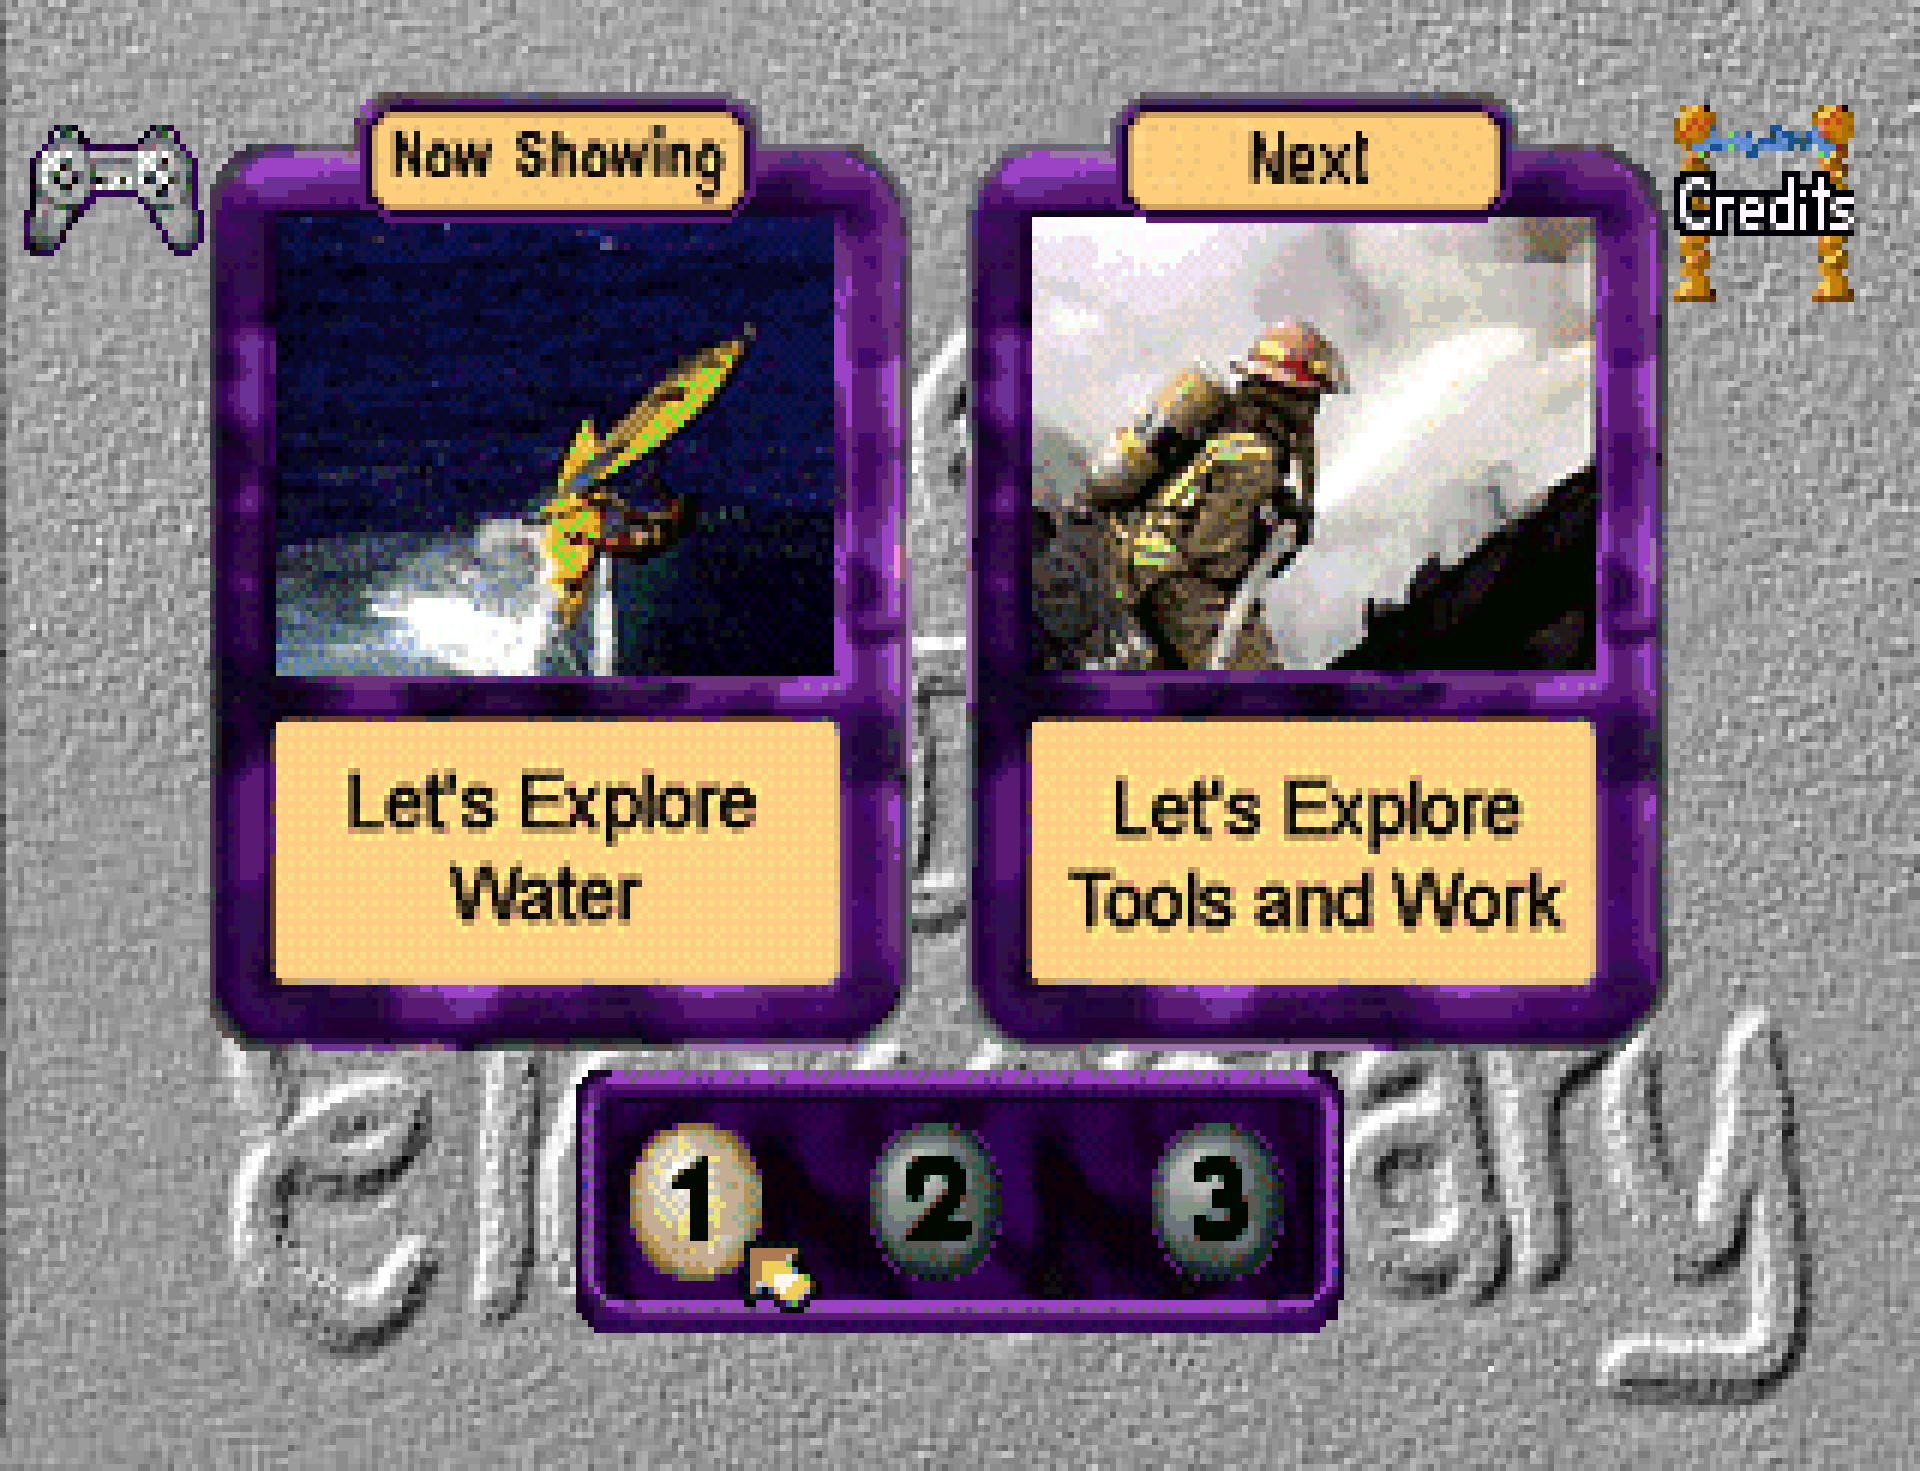
\includegraphics[width=\linewidth]{Games/ScienceIsElementary/Images/ScienceIsElementary2Image1.png}
        \caption{Science Is Elementary 2 - Screenshot 1}
    \end{subfigure}
    \begin{subfigure}{0.45\textwidth}
        \centering
        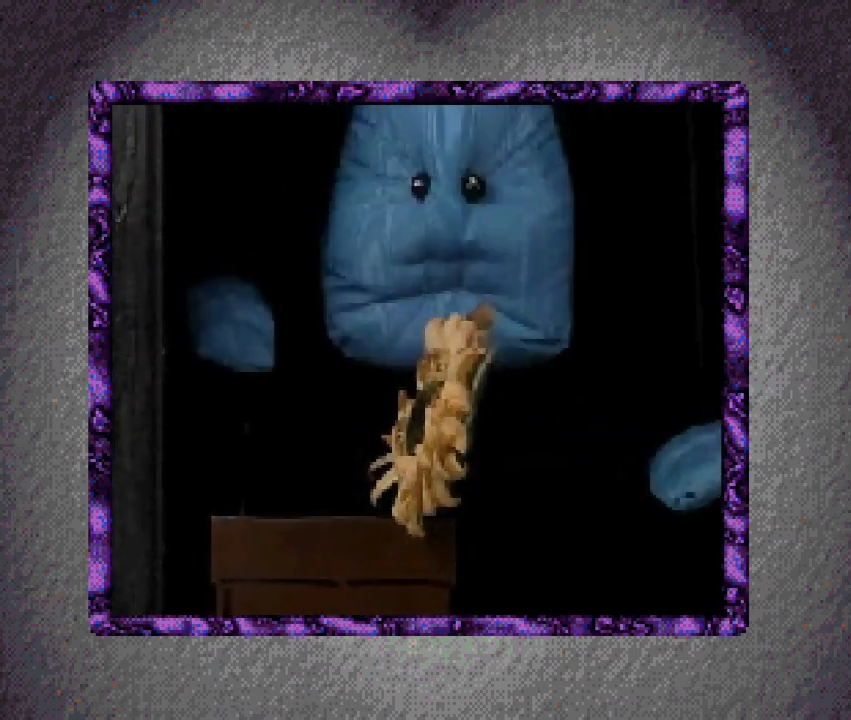
\includegraphics[width=\linewidth]{Games/ScienceIsElementary/Images/ScienceIsElementary2Image2.png}
        \caption{Science Is Elementary 2 - Screenshot 2}
    \end{subfigure}

    \begin{subfigure}{0.45\textwidth}
        \centering
        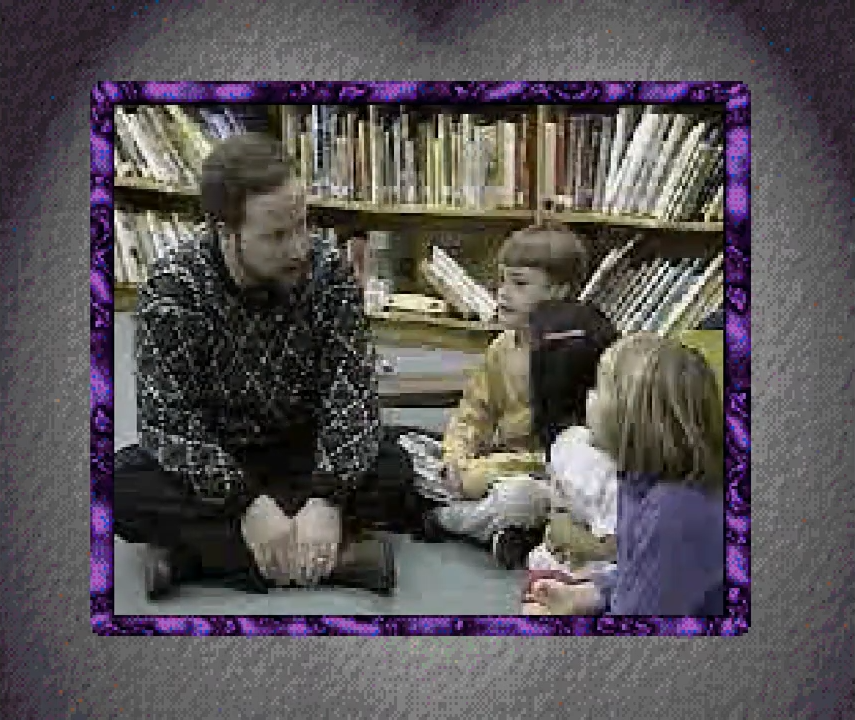
\includegraphics[width=\linewidth]{Games/ScienceIsElementary/Images/ScienceIsElementary2Image3.png}
        \caption{Science Is Elementary 2 - Screenshot 3}
    \end{subfigure}
    \begin{subfigure}{0.45\textwidth}
        \centering
        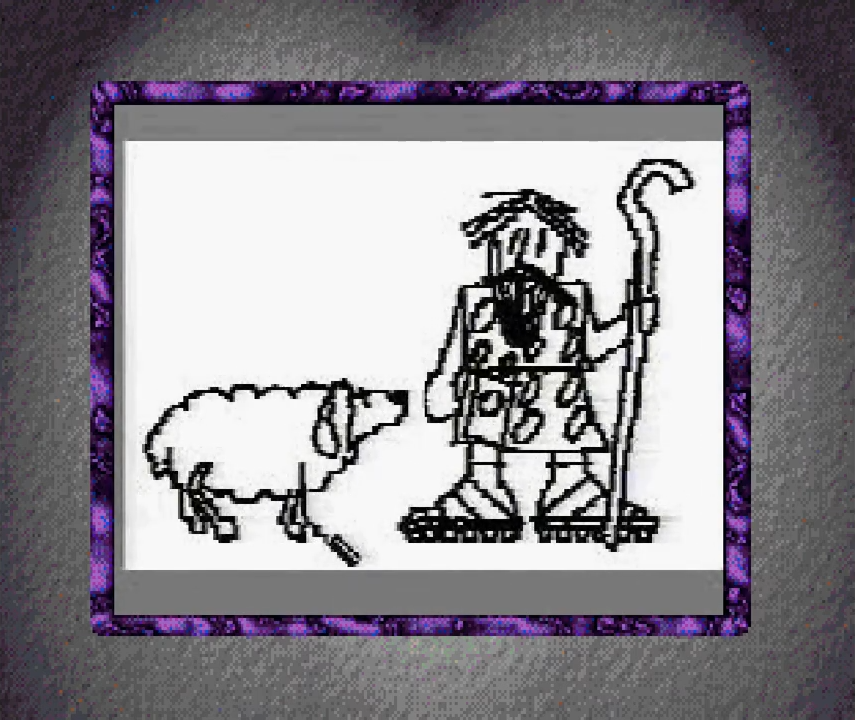
\includegraphics[width=\linewidth]{Games/ScienceIsElementary/Images/ScienceIsElementary2Image4.png}
        \caption{Science Is Elementary 2 - Screenshot 4}
    \end{subfigure}
    \caption{Screenshots from Science Is Elementary 2}
\end{figure}